% Generated by scripts/md_to_latex.py --ieee from paper_ieee_full.md.
% Do not edit by hand: change the markdown (checked by verify_draft.py's subset mode) and regenerate.
\documentclass[conference]{IEEEtran}
\IEEEoverridecommandlockouts
\pdfinfoomitdate=1
\pdftrailerid{}
\pdfsuppressptexinfo=-1
\usepackage[T1]{fontenc}
\usepackage{amsmath,amssymb}
\usepackage{graphicx}
\usepackage{booktabs}
\usepackage{array}
\usepackage[numbers,sort&compress]{natbib}
\usepackage{url}
\usepackage[hidelinks]{hyperref}
\setlength{\emergencystretch}{1.5em}

\title{Knowledge the Network Already Has: An Exogeneity Precondition for Neuro-Symbolic Intrusion Detection}
\author{\IEEEauthorblockN{Anonymous Authors}\IEEEauthorblockA{Under review}}

\begin{document}
\maketitle

\begin{abstract}
Neuro-symbolic intrusion detectors that report gains from injected knowledge tend to share a property that is rarely stated: the knowledge they add is information the neural network could not compute from its input. Our own system, a 1D CNN with Logic Tensor Network axioms over CIC-IDS2017 flow features, did not have this property, and its axioms were worse than the same trainer run without them in all 17 CNN training runs we paired them with. We argue that symbolic knowledge can help only to the extent that it lies outside the model's learned feature basis, and test how far the same condition explains a second failure: every Bot flow is classified as benign in all 17 runs, although an oracle reaches a PR-AUC of 0.9988 from the same features. We then show that the benchmark cannot host the experiment published gains rely on, because host-role knowledge derived from the capture is predictable from the flow features (AUC 0.990-0.994). Re-examining the neuro-symbolic system our work started from, we find that its reported gain does not appear against a matched control (+0.55 against +12.13 percentage points). All results are paired on seed under deterministic training, and the pipeline reproduces from the raw data.
\end{abstract}

\begin{IEEEkeywords}
Intrusion detection, neuro-symbolic learning, zero-day attacks, CIC-IDS2017, Logic Tensor Networks, reproducibility
\end{IEEEkeywords}

\section{Introduction}\label{sec:1}

A common argument for neuro-symbolic learning is that domain knowledge written as logic can make up for what the training data lacks. Intrusion detection looks like a good place to test this. A data-driven detector is weakest on attacks that never appeared in training, and those are the cases where knowledge about how networks and attacks behave should matter most.

We built a neuro-symbolic intrusion detector to test the idea, and it did not work. Its Logic Tensor Network axioms encode behaviours such as burst traffic, packet-size variance and destination ports outside the standard service ports. Alone they changed macro zero-day PR-AUC by $-$0.0004, which is not significant. Compared with the same trainer run without axioms, they made the system worse with every one of the 17 CNN training runs we paired them with, whether or not a knowledge-graph channel was added. This paper sets out to explain that outcome, and we think the explanation applies beyond our system.

Published systems that do report gains have something ours did not. \citet{grov2024} add a single axiom stating that flows which do not involve a web server cannot be web attacks, and roughly double their web-attack precision. KnowGraph \citep{zhou2024} reasons over relations between entities and raises the true-positive rate from 0.0 \% to 35.5 \% at a 0.5 \% false-positive rate, a setting in which the neural baseline detects nothing. \citet{kalutharage2025} map alerts onto an external attack taxonomy. In all three, the added knowledge is something the network could not have worked out from its own input. Each of our behaviour predicates, in contrast, is a fixed function of flow features the network already reads, so at most it could act as an inductive bias. It could not add evidence.

We state this as a precondition: symbolic knowledge helps a neural detector to the extent that it lies outside the model's learned feature basis. The paper makes four contributions around it.

\begin{enumerate}
  \item \textbf{One principle, and how far it reaches (Sections~\ref{sec:3}--\ref{sec:4}).} Knowledge that falls inside the learned basis adds nothing. We ask whether the same condition explains attack families that are absent from training: our CNN never reaches Bot, whose discriminative features are not among those the known-class task relies on. A tuned random forest reaches Bot in part without relying more on those features, so overlap is an account of the CNN's failure, not a general law.
  \item \textbf{A durability test (Section~\ref{sec:5}).} The unreachability survives five separate attempts to break it: a capture in which the family is plentiful, corrected labels, an explicitly trained reject class, cross-dataset augmentation, and a sweep over architectures and out-of-distribution scorers.
  \item \textbf{A negative result on evaluability (Section~\ref{sec:6}).} Host-role knowledge built from metadata that the network never sees can still be recovered from the network's features. A benchmark without an external knowledge artefact cannot host the experiment on which published neuro-symbolic gains depend.
  \item \textbf{A controlled re-examination of the base system (Section~\ref{sec:7}).} The satisfiability gain of the neuro-symbolic system our work started from does not appear against a matched control, and our apparent agreement with its CNN does not survive population matching.
\end{enumerate}

\begin{figure*}[t]
\centering
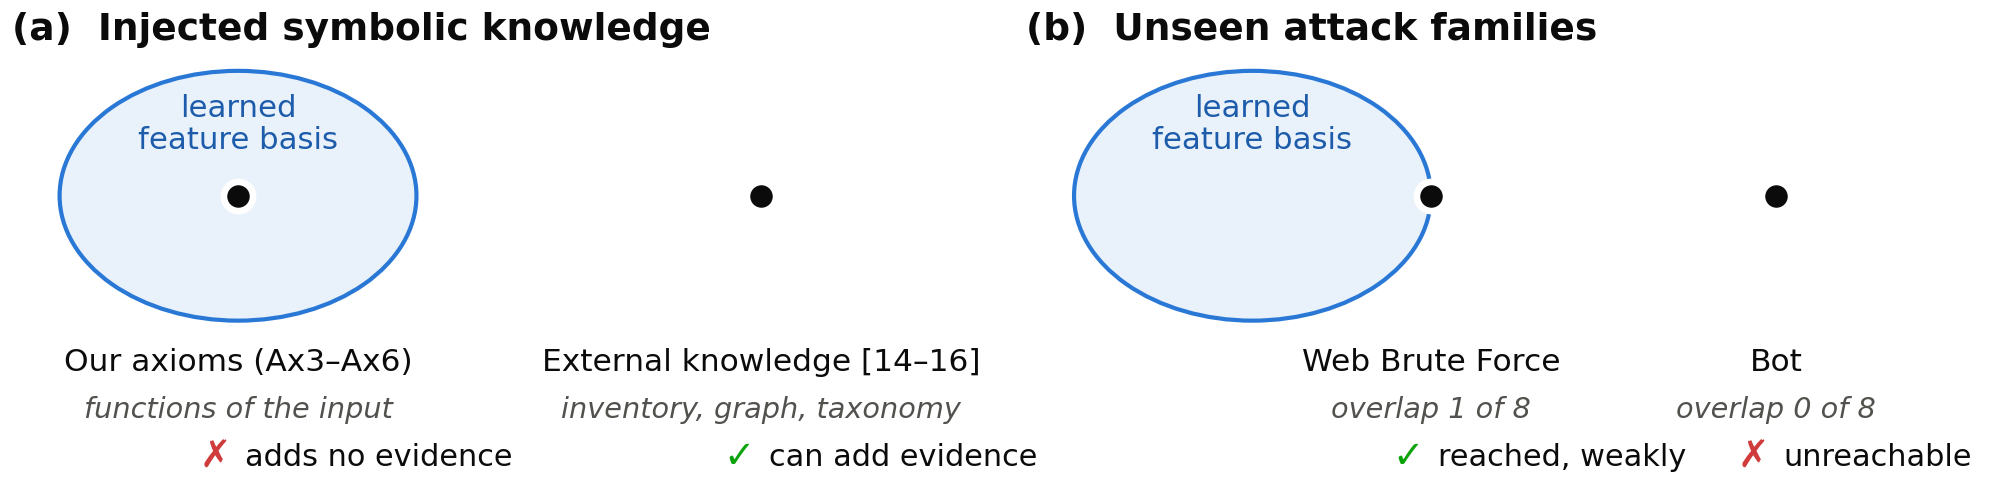
\includegraphics[width=\textwidth]{figures/nesy_fig1_thesis}
\caption{\emph{One principle, two consequences.} Both panels show the same learned feature basis, that is, the features a closed-set objective selects. (a) Symbolic knowledge can only help from outside the basis. Our Logic Tensor Network axioms are functions of the flow features and add no evidence, while the knowledge used in published systems \citep{grov2024,zhou2024,kalutharage2025} cannot be computed from the input. (b) Our account of unseen families: a family is reached as far as it overlaps the basis. Web Brute Force shares 1 of 8 discriminative features and is reached only weakly once label artefacts are removed (Section~\ref{sec:8}). Bot shares none and is not reached by the CNN. A tuned random forest reaches Bot in part without relying more on its features (Section~\ref{sec:4}), so panel (b) describes our CNN rather than every model. Note that inside and outside lead to opposite outcomes in the two panels.}\label{fig:thesis}
\end{figure*}

Two measurement problems limit the magnitudes we can report (Section~\ref{sec:8}), and we show both on our own system. The metric most papers report cannot separate methods by zero-day ability. In addition, once the labels are corrected, two of our three main zero-day families turn out to have been measuring whether the dataset labels a failed connection attempt as an attack. These problems cap what we can claim about effect sizes, but they do not affect the CNN's failure on Bot.

\section{Setting and measurement}\label{sec:2}

\textbf{Data.} We use the CIC-IDS2017 \citep{sharafaldin2018} flow features, 68 numeric features per flow. Nine attack families and benign traffic are treated as known. They are split 80/10/10 with stratification, and benign traffic is under-sampled to a 1:1 ratio, giving 883,796 training, 110,475 validation and 114,658 test flows. Six rare families (Bot, Heartbleed, Infiltration, and Web Attack Brute Force, XSS and SQL Injection) occur only in the test set. Under-sampling benign traffic raises the attack base rate about fourfold, so absolute PR-AUC values here are higher than they would be at the capture's own prevalence (Section~\ref{sec:11}).

\textbf{Metric.} Our main metric is macro zero-day PR-AUC over the three unseen families with enough samples: Bot (n = 1,956), Web Attack Brute Force (n = 1,507) and Web Attack XSS (n = 652). Heartbleed (n = 11), Infiltration (n = 36) and SQL Injection (n = 21) are too small and are left out. PR-AUC cannot fall below the prevalence of the positive class, so when test sets differ in prevalence (between datasets or between labellings) we compare lift, defined as PR-AUC divided by prevalence. A random ranker has a lift of 1.0.

\textbf{Reproducibility.} Without determinism flags, training at a fixed seed does not give identical results, so we measured run-to-run variation before comparing any methods. The standard deviation is 0.0222 from nondeterminism alone, 0.0171 across seeds with determinism enabled (n = 6) and 0.0228 across data splits, which puts the uncertainty on a single absolute number at about 0.0285. All comparisons are paired on seed. We call a difference established only if its sign is the same on every seed, and we give magnitudes as ranges. This procedure led us to withdraw one of our own earlier claims: a gap of 0.9 SD that a paired bootstrap had reported as significant (p = 0.001).

\section{A symbolic pillar that could not help}\label{sec:3}

\textbf{Architecture.} The system has three parts: a 1D CNN over the flow features, a Logic Tensor Network \citep{badreddine2022} layer that grounds fuzzy axioms in network behaviours, and a knowledge-graph channel that scores how quickly clusters of flows grow over time. The axioms (Ax3--Ax6) tie the network's attack output to behaviour predicates such as large packets with high size variance, bursts, scan-like probing and a destination port outside a list of standard service ports (\texttt{BeaconLike}).

\textbf{Results.} We tried injecting the axioms at the loss, at the representation and at inference. In every case the symbolic component either lowered macro zero-day PR-AUC or left it unchanged. On its own it contributes $-$0.0004 (n.s.). The cleaner test holds everything but the axioms fixed: the same trainer with the axiom weight at zero. Against it, the axioms lower macro zero-day PR-AUC with each of the 11 CNN runs trained before our determinism controls (by 0.0062 on average) and each of the 6 trained after (0.0068), and by more when a knowledge-graph channel is also fused (0.0212 and 0.0324). An earlier version of this comparison, which added the axioms on top of a knowledge-graph fusion built on three CNN runs, reported a significant loss; that fusion does not hold across CNN runs (Section~\ref{sec:8}), so we report the matched comparison instead. One axiom seemed at first to help on Bot, but the effect disappeared when we repeated the experiment over several seeds. Because the sign of the effect is the same in every configuration, we do not think better tuning would change the conclusion.

Comparing our system with published ones that report gains suggests why:

\begin{center}\footnotesize
\begin{tabular}{@{}>{\raggedright\arraybackslash}p{\dimexpr 0.220\linewidth-2\tabcolsep\relax}>{\raggedright\arraybackslash}p{\dimexpr 0.455\linewidth-2\tabcolsep\relax}>{\raggedright\arraybackslash}p{\dimexpr 0.325\linewidth-2\tabcolsep\relax}@{}}
\toprule
\textbf{system} & \textbf{knowledge injected} & \textbf{computable from the flow features?} \\
\midrule
\citet{grov2024} & flows not involving a web server are not web attacks & no, needs an asset inventory \\
KnowGraph \citep{zhou2024} & logic over relations between entities & no, needs a relational graph \\
\citet{kalutharage2025} & mapping of techniques to an attack taxonomy & no, needs an external taxonomy \\
ours & behaviour predicates (Ax3--Ax6) & yes, each is a function of the input \\
\bottomrule
\end{tabular}
\end{center}

All seven of our behaviour predicates are deterministic functions of features the network already consumes. \texttt{HighEntropy}, for example, is the standard deviation of packet length rather than Shannon entropy, and \texttt{BeaconLike} depends on the destination port. \texttt{BeaconLike} was also selected by testing candidate encodings against Bot flows, which belong to a zero-day family, so it is not a clean test of transfer to unseen attacks. The axioms made no positive difference, so this weakens nothing we conclude, but a positive result from it would not have counted. A predicate that the network can compute for itself carries no new information. The most it can do is reshape the hypothesis space, which is a form of regularisation. In short, the knowledge we injected was endogenous.

This leads to the precondition we propose: \emph{symbolic knowledge helps a neural detector to the extent that it lies outside the model's learned feature basis.} The next section shows that the same condition also accounts for a failure that at first seems unrelated.

\section{One principle, two consequences}\label{sec:4}

A closed-set discriminative model learns the features that separate the classes in its training objective and has no reason to learn others. It follows that a class the model has never seen can be reached only as far as that class's signature overlaps the learned basis. This is the precondition of Section~\ref{sec:3} again, with an unseen class in the place of an injected predicate. When the overlap is empty, nothing in the training objective constrains the model's output on the class.

Bot is a case where the overlap appears to be empty, and we use it to test this account:

\begin{itemize}
  \item In all 17 CNN training runs, 100 \% of Bot flows are classified as BENIGN, with a mean p(BENIGN) of at least 0.998 in every run. The model is not uncertain about Bot; it is confidently wrong, so confidence-based rejection methods have nothing to work with.
  \item The eight features that best separate Bot from benign traffic have 0 of 8 in common with the eight that a gradient-boosted model of the known-class task uses most. This belongs to that model's importance ranking rather than to the task: two random forests trained on the same task each have 2 of the 8 among their own top eight.
  \item Bot is the family whose ranking agrees least between training runs (Figure~\ref{fig:mechanism}). Over all 15 pairs of six deterministic CNN runs, the median Spearman correlation on Bot flows is +0.55, and single pairs range from $-$0.52 to +0.92; the web families have medians of +0.81 and +0.93. The 11 runs trained before we enabled determinism look the same (median +0.59). The three runs we first analysed gave $-$0.090, the low end of this range rather than its typical value, and we no longer describe the Bot ranking as noise. Nor is the inconsistency a property of closed-set training in general. A random forest with default feature sampling shows it ($\rho$ = 0.068), but with the number of features per split selected on validation the same forest gives +0.923 and ranks Bot at 6.4 times chance.
  \item The information is available in the features. An oracle trained with Bot labels reaches a PR-AUC of 0.9988 from the same inputs. It uses zero-day labels and so is an upper bound rather than a usable method, but it shows that the obstacle is the lack of supervision, not missing information or the choice of input modality.
\end{itemize}

\begin{figure*}[t]
\centering
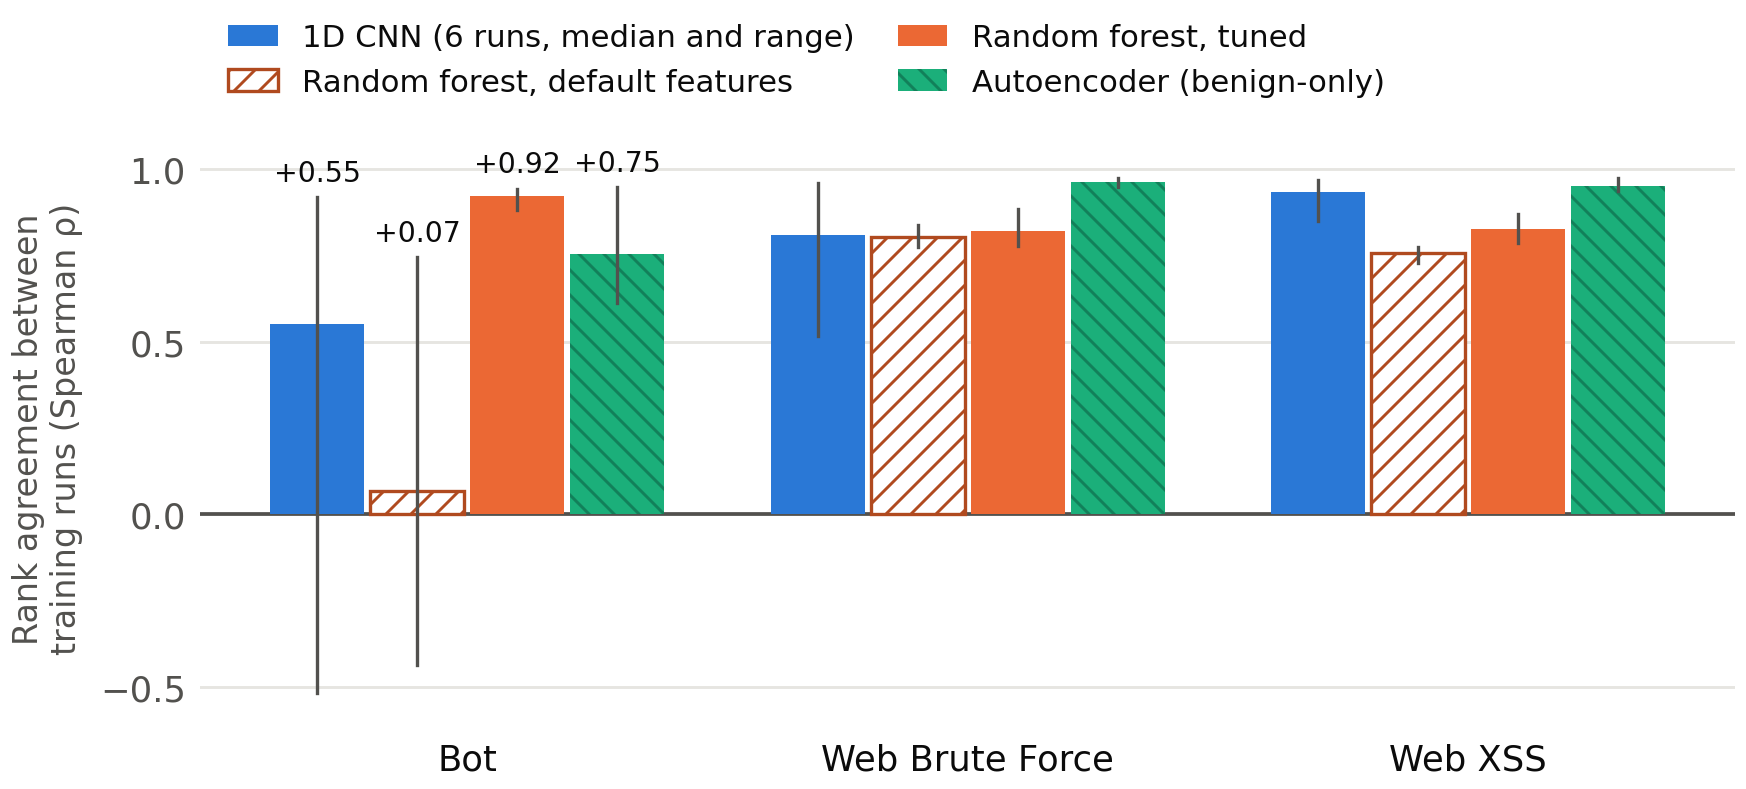
\includegraphics[width=\textwidth]{figures/nesy_fig2_mechanism}
\caption{\emph{Agreement between training runs, by family.} Each bar shows how well a model's ranking of one unseen family's test flows agrees between training runs (Spearman $\rho$), and each line shows the range over pairs of runs. The CNN bar is the median over all 15 pairs of six deterministic runs; the forests and the autoencoder have three runs each. Bot is the CNN's least consistent family and its most variable one. A random forest with default feature sampling is also inconsistent on Bot, but the same forest with its feature sampling selected on validation is the most consistent model on Bot, so the inconsistency depends on the model's configuration and not only on closed-set training.}\label{fig:mechanism}
\end{figure*}

Taken together, knowledge that lies inside the basis (our axioms) adds no evidence, and a class that lies outside it (Bot) is not reached by the CNN. Both are consistent with what a closed-set objective does and does not constrain. A tuned random forest reaches Bot partially, and the account predicts that it should rely on Bot's features more than the untuned forest does. We specified this test before running it, and it failed: the tuned forest puts less of its importance on Bot's eight features (0.19 against 0.21, lower on every seed) and more on the eight known-class features (0.39 against 0.24). Overlap as we measure it therefore does not decide which models reach Bot, and we offer the account as an explanation of the CNN's failure rather than as a general law. The evidence is stronger for the unreachable case than for the reachable one (Section~\ref{sec:8}). Our support for the claim that overlapping families are reached came from web-attack scores, and most of those scores disappear under corrected labels. The ordering between families holds; the sizes of the scores do not.

\section{Durability: five attempts to break it}\label{sec:5}

A single demonstration of a mechanism is not strong evidence, so we tried to break it in five ways. For each attempt we wrote down, before running it, what result would count against the mechanism.

\begin{center}\footnotesize
\begin{tabular}{@{}>{\raggedright\arraybackslash}p{\dimexpr 0.392\linewidth-2\tabcolsep\relax}>{\raggedright\arraybackslash}p{\dimexpr 0.217\linewidth-2\tabcolsep\relax}>{\raggedright\arraybackslash}p{\dimexpr 0.392\linewidth-2\tabcolsep\relax}@{}}
\toprule
\textbf{attempt} & \textbf{what it rules out} & \textbf{result for Bot} \\
\midrule
Independent capture (CSE-CIC-IDS2018), training size matched & Bot is merely rare & Bot is common there and scores 0.83$\times$ chance, worse than a random ranker \\
Corrected labels \citep{engelen2021}, attack flows without payload removed & a labelling artefact & the remaining Bot flows (n = 738) give lifts of 0.57 / 0.64 / 8.99; two of three seeds are below chance \\
Reject class: three known families merged into \texttt{UNKNOWN} & the model was never trained to reject & at best chance level (+0.068), with the sign changing between seeds \\
Cross-dataset augmentation with the 2018 known classes & the basis was too narrow & $-$0.1461 macro against a seed-matched control; better on 0/3 seeds \\
Sweep over 4 deep architectures, 7 classical models, 4 benign-only models and 9 OOD scorers & the choice of method & no method in the sweep reaches Bot (a validation-tuned random forest does in part, Section~\ref{sec:4}); the best OOD scorer gets 0.0783 against a threshold of 0.08 fixed in advance (0.0576 on deterministic re-runs) \\
\bottomrule
\end{tabular}
\end{center}

The corrected-label experiment is the hardest test, and the way it fails deserves a comment. Our criterion was a lift above chance on every seed. The mean lift is 3.4$\times$, which on its own would look like detection, but no individual run is close to that value. The large spread between seeds matches the variable Bot ranking described in Section~\ref{sec:4}.

The reject-class experiment gave the clearest positive evidence. We ran two versions that differ only in which known families are merged into \texttt{UNKNOWN}, and they produce a double dissociation that holds on every seed and for every family. Merging three similar DoS variants ranks Bot below chance ($-$0.206) while giving the best scores on the web families. Merging three dissimilar families reverses both effects, and the difference on Bot is +0.274 (2.57$\sigma$, 3/3 seeds). A reject class is therefore not a neutral ``none of the above'' category. What it can reach depends on the features of the classes merged into it, which is the mechanism of Section~\ref{sec:4} appearing in an open-set setting. For Bot, chance level remains the upper limit.

Augmentation failed for a different reason. Adding a related attack family from the other capture sharpened one decision region until it began to fire on benign traffic from the original capture. The number of benign flows scoring above the median Web Brute Force flow rose from 2 to 242, and 81 \% of them were assigned to \texttt{SSH-Patator}. Widening the basis along directions it already covered added false positives, not new reach.

\section{Evaluability: the benchmark cannot supply exogenous knowledge}\label{sec:6}

If the precondition in Section~\ref{sec:3} is correct, the obvious next step is to inject knowledge from outside the basis. We tried to do this on CIC-IDS2017, and the attempt failed before any injection, at the stage of checking that the knowledge was actually exogenous. We report that failure as a result.

\textbf{Construction.} Source and destination IP addresses are not among the model's features, and a single flow's feature vector cannot describe how a host behaves across many flows. We therefore derived host-role predicates from the flow metadata: whether a destination normally serves a given port, whether a flow's port is unusual for its host, how many destinations a source contacts, and how persistent a source-destination pair is. The host profiles use training flows only, so the construction is inductive. We deliberately left out attacker identity. The testbed documentation lists the attacker subnet, and conditioning on it would amount to label leakage presented as domain knowledge.

\textbf{Testing the premise.} A predicate is exogenous only if the network could not already compute it. To check this, we trained gradient-boosted models to predict each predicate from the flow features:

\begin{center}\footnotesize
\begin{tabular}{@{}>{\raggedright\arraybackslash}p{\dimexpr 0.333\linewidth-2\tabcolsep\relax}>{\raggedleft\arraybackslash}p{\dimexpr 0.244\linewidth-2\tabcolsep\relax}>{\raggedleft\arraybackslash}p{\dimexpr 0.423\linewidth-2\tabcolsep\relax}@{}}
\toprule
\textbf{predicate} & \textbf{all features} & \textbf{without \texttt{Destination Port}} \\
\midrule
Unusual port for host & AUC 0.990 & 0.988 \\
Host serves a web port & AUC 0.994 & 0.992 \\
Source fan-out & R$^{2}$ 0.949 & 0.898 \\
Pair persistence & R$^{2}$ 0.914 & 0.886 \\
\bottomrule
\end{tabular}
\end{center}

None of the predicates is exogenous. The ablation matters here. Removing the port feature hardly changes the scores, so the result is not just the flow's own port revealing the answer; the other features are enough to determine host role and cross-flow structure. In a testbed where each host runs one scripted role, the characteristics of a flow nearly identify the host, and with it the host's aggregate properties.

\textbf{What generalises.} Knowledge obtained by aggregating the same data is not exogenous. The axiom of Grov et al. works because their asset inventory comes from outside the traffic capture. Ours was inferred from the capture, and whatever can be inferred from the capture can largely be inferred from its features as well. CIC-IDS2017 comes with no asset inventory, topology or threat intelligence, so neuro-symbolic methods of the kind used in the literature cannot be properly evaluated on it. For this reason we did not run the injection experiments: injecting a predicate the model can already compute would present feature engineering as a symbolic result. The thresholds we used (AUC $<$ 0.75, R$^{2}$ $<$ 0.5) are conventions, and a predicate at R$^{2}$ = 0.90 still leaves some variance unexplained. A stronger predictor, however, could only make the conclusion stronger.

\section{Re-examining the base paper}\label{sec:7}

Our work started from \citet{bizzarri2024}, who trained a Logic Tensor Network on CIC-IDS2017 with a combined cross-entropy and satisfiability loss and reported better accuracy on unknown attacks. We re-examined that result with controls it did not have.

\textbf{The gain does not appear against a matched control.} We trained their loss (cross-entropy plus the satisfiability term at $\omega$ = 1) and a matched control with the term switched off ($\omega$ = 0), identical in every other respect, with three deterministic seeds each. The satisfiability term changes zero-day accuracy by +0.55 percentage points (+0.60, $-$0.84 and +1.89 on the three seeds), against the +12.13 they report, and changes macro zero-day PR-AUC by $-$0.0090, better on 1 seed of 3. Neither change is consistent in direction.

\textbf{The reported gain is a change of operating point.} Across the five evaluation views, the hybrid LTN model improves on the 1D CNN by +0.09, +0.15, +0.07 and +2.15 percentage points on the four views that contain benign traffic, and by +12.13 points on the one view that does not. On the nine known classes the hybrid model makes 452 false positives against the CNN's 380. The satisfiability term penalises calling an attack benign, so it moves the decision boundary towards the attack class. Their zero-day view contains only attack rows, so precision is always 1, accuracy equals recall, and F1 = 2A/(1+A); a model that flags every flow as an attack would score 100 \% on both.

\textbf{One connection, and a coincidental agreement.} Heartbleed is 42.2 \% of their zero-day set, and all 11 Heartbleed flows in CIC-IDS2017 share one 5-tuple and fall within 20 minutes, so the largest component of the reported zero-day score is one network event. On their zero-day view our CNN scores 47.85 \% against their 48.34 \%. They delete payload-less records and we do not; on the corrected-label release with the attempted, payload-less flows removed, which is the closest analogue of their filtering, our CNN's view-5 accuracy is 0.69 \% (0.82, 0.82 and 0.41 \% over three seeds). Our 47.85 \% came from failed connection attempts labelled as attacks.

\textbf{Their class balancing.} Under their rule, every known attack class cut to the size of the smallest (4,399 training flows each), our CNN's macro zero-day PR-AUC falls from 0.6299 to 0.4699; a training set of the same size with the natural class mix scores 0.2118, below the balanced one on every seed. With the natural mix at this size the two slow-rate DoS classes keep only 350 and 369 training flows and the web attacks are classified as benign instead of being absorbed into them. Balancing does not account for their zero-day accuracy either: on view 5 our balanced CNN scores 45.10 \%, against 47.56 \% on our own split.

\section{What limits the magnitudes}\label{sec:8}

Two measurement problems limit how much weight any of our numbers can bear. We report both, and the second one removes two of our own main zero-day families from consideration.

\textbf{Label semantics.} \citet{engelen2021} reprocessed CIC-IDS2017 with a corrected flow meter and added an \texttt{X -- Attempted} label for attack flows that carried no payload. About two-thirds of Bot flows and about nine-tenths of the web-attack flows fall into this category. After retraining on the corrected release we obtain:

\begin{center}\footnotesize
\begin{tabular}{@{}>{\raggedright\arraybackslash}p{\dimexpr 0.271\linewidth-2\tabcolsep\relax}>{\raggedleft\arraybackslash}p{\dimexpr 0.271\linewidth-2\tabcolsep\relax}>{\raggedleft\arraybackslash}p{\dimexpr 0.260\linewidth-2\tabcolsep\relax}>{\raggedleft\arraybackslash}p{\dimexpr 0.198\linewidth-2\tabcolsep\relax}@{}}
\toprule
\textbf{family} & \textbf{attempted folded in} & \textbf{attempted excluded} & \textbf{n (excluded)} \\
\midrule
Web Attack Brute Force & 29.4$\times$ & 2.1$\times$ & 151 \\
Web Attack XSS & 61.5$\times$ & \emph{unmeasurable} & 27 \\
\bottomrule
\end{tabular}
\end{center}

When flows that transmitted nothing are removed, the PR-AUC for Web Brute Force drops from 0.8861 to 0.0072. Much of the apparent detection was detection of bare connection attempts, which look very different from normal traffic. Measuring a mislabelled benchmark with a better metric does not fix the labels. This is why the reachable case in Section~\ref{sec:4} is weak. The unreachable case is unaffected, because Section~\ref{sec:5} tested it on these corrected labels.

\textbf{Metric resolution.} The metric the field usually reports does not resolve the capability it is used to support. Across 31 methods evaluated under the same protocol, 37 of 169 method pairs (22 \%) cannot be told apart statistically on this metric even though their macro zero-day PR-AUC differs by a factor of two or more. In the most extreme pair, the two methods are 0.0052 apart on the reported metric and 16.6$\times$ apart on zero-day performance. The metric is neither noisy nor unrelated to zero-day performance ($\rho$ = +0.582); it is simply too coarse in the range where results are reported.

\textbf{A component that appeared to help, withdrawn.} Fused with our three reference CNN runs, the knowledge-graph channel, which scores cluster growth over time, raised macro zero-day PR-AUC, and the gain held when its number of clusters was selected on one half of the test set and reported on the other (+0.0305 at 2.86$\sigma$). It does not hold across a wider set of CNN runs. Fused with each of 11 training runs of the same CNN configuration, the online variant improves on its own CNN run in 5 of the 11, and in 0 of the 6 deterministic re-runs. The gain follows where each CNN run happens to rank one web-attack family among all test flows (Spearman +0.95), a property that varies between runs of one configuration and that no per-family score reveals. The gain belonged to three runs rather than to the method, and we withdraw it. With it withdrawn, no component of our architecture has been shown to improve on the neural baseline.

\section{Related work}\label{sec:9}

\textbf{Neuro-symbolic intrusion detection.} Logic Tensor Networks \citep{badreddine2022} provide the machinery for turning fuzzy logic into a loss. \citet{bizzarri2024} applied it to CIC-IDS2017 with a combined cross-entropy and satisfiability loss and reported better accuracy on unknown attacks. Section Section~\ref{sec:7} re-examines that result under a matched control. As we read them, the gains reported in \citep{grov2024,zhou2024,kalutharage2025} come from exogenous knowledge. We do not criticise those papers, since their knowledge really is exogenous. Our point is that this property does the work and is usually left implicit, and without it a reader cannot tell a knowledge result from a feature-engineering result. We state the property, test it, and show that a widely used benchmark cannot satisfy it. A recent survey \citep{hakim2025} also observes that evaluation gaps limit most neuro-symbolic cybersecurity studies.

\textbf{The benchmark.} Many papers report results on CIC-IDS2017 \citep{sharafaldin2018}. \citet{engelen2021} documented problems in its flow construction and labelling and released corrected processing, a follow-up study measured the effect on detection results \citep{lanvin2023}, and a survey of 89 intrusion datasets argues that data quality is now a limiting factor for the field \citep{goldschmidt2025}. We add a consequence specific to zero-day detection, and point out a further gap: the benchmark provides no external knowledge artefact.

\textbf{Closed worlds and machine learning for security.} \citet{sommer2010} argued that intrusion detection is a difficult setting for machine learning because the events of interest lie outside the closed world of the training data. Section~\ref{sec:4} gives a mechanism for one instance of this, in which the failure takes the form of confident misclassification. \citet{arp2022} list ten common pitfalls in machine learning for security. Of the ten, lab-only evaluation is not addressed here, and the threat model only in part (Section~\ref{sec:11}).

\textbf{Open-set recognition and OOD scoring.} Unseen attacks have long been treated as an open-set recognition problem \citep{cruz2017}, and post-hoc scorers do so without retraining \citep{hendrycks2017,liang2018,liu2020}. None of them helps on Bot (Section~\ref{sec:5}).

\section{Reproducibility}\label{sec:10}

Training is deterministic: two full 50-epoch runs with the same seed produce byte-identical output. We ran the whole pipeline from the raw CSVs into an empty directory. It completed 20 of the 26 stages in 6.5 hours, and 72 files are byte-identical to the artifacts behind this paper, including the split, all three CNN seeds with their embeddings, all three autoencoders and every knowledge-graph seed; four differ only at float level and nothing differs otherwise. The six incomplete stages need records from experiments outside the pipeline. Every number in the paper is checked mechanically against the per-run records. Code, configuration and records are released; the dataset and trained weights are not.

\section{Limitations and conclusion}\label{sec:11}

\textbf{Limitations.} Our two captures come from the same producer and use related methods, so they do not show that the findings generalise to other network environments. Under corrected labels only two zero-day families have enough samples. We use flow features rather than payload bytes throughout, although the oracle result suggests that modality is not the obstacle. The thresholds in our exogeneity test are conventions. A bounded, non-adaptive evasion test finds that timing jitter lowers the CNN's macro zero-day PR-AUC to 0.5620, while every perturbation we tried raises the scores of the autoencoder and the tuned forest; we do not evaluate an adaptive adversary, and the system has not been deployed. Benign traffic is under-sampled 4.11-fold, as in the base paper, so absolute PR-AUC is optimistic: at the capture's own benign proportion the CNN's macro zero-day PR-AUC is 0.5845, not 0.6299. The split is stratified at random over a chronologically ordered capture and is not grouped by connection. Grouping by connection lowers the CNN's macro zero-day PR-AUC from 0.6299 to 0.5589, and a chronological split halves the benign-only autoencoder's score.

\textbf{Conclusion.} Symbolic knowledge helps a neural intrusion detector to the extent that it lies outside the model's learned feature basis. The same condition accounts for our CNN's failure on an attack family whose features it does not use, a failure that held under every test we designed to break it, although a tuned random forest shows that overlap alone does not decide which models reach such a family. The neuro-symbolic systems that report gains use knowledge that is truly exogenous. Ours did not, and on CIC-IDS2017 we could not construct any, because knowledge aggregated from a capture can be recovered from that capture's features. We suggest that anyone reporting a neuro-symbolic gain should first check that the injected knowledge is not already present in the input, and should be aware that some benchmarks make this impossible.

\emph{Code, configuration and per-run records are released with this paper; the dataset and trained weights are not (Section~\ref{sec:10}).}

\bibliographystyle{IEEEtranN}
\bibliography{refs}

\end{document}
